% Fig. 1 -- Concept of BeeMove: from bench video to walking-path analytics,
% with the active-learning loop that customises the detector.
% Build: pdflatex Fig1.tex  (or `make figures` at the project root)
\documentclass[tikz,border=2pt]{standalone}
\usepackage[T1]{fontenc}
\usepackage[scaled=0.92]{helvet}
\renewcommand{\familydefault}{\sfdefault}
\usetikzlibrary{arrows.meta,positioning,fit,backgrounds,calc,shapes.geometric}

\begin{document}
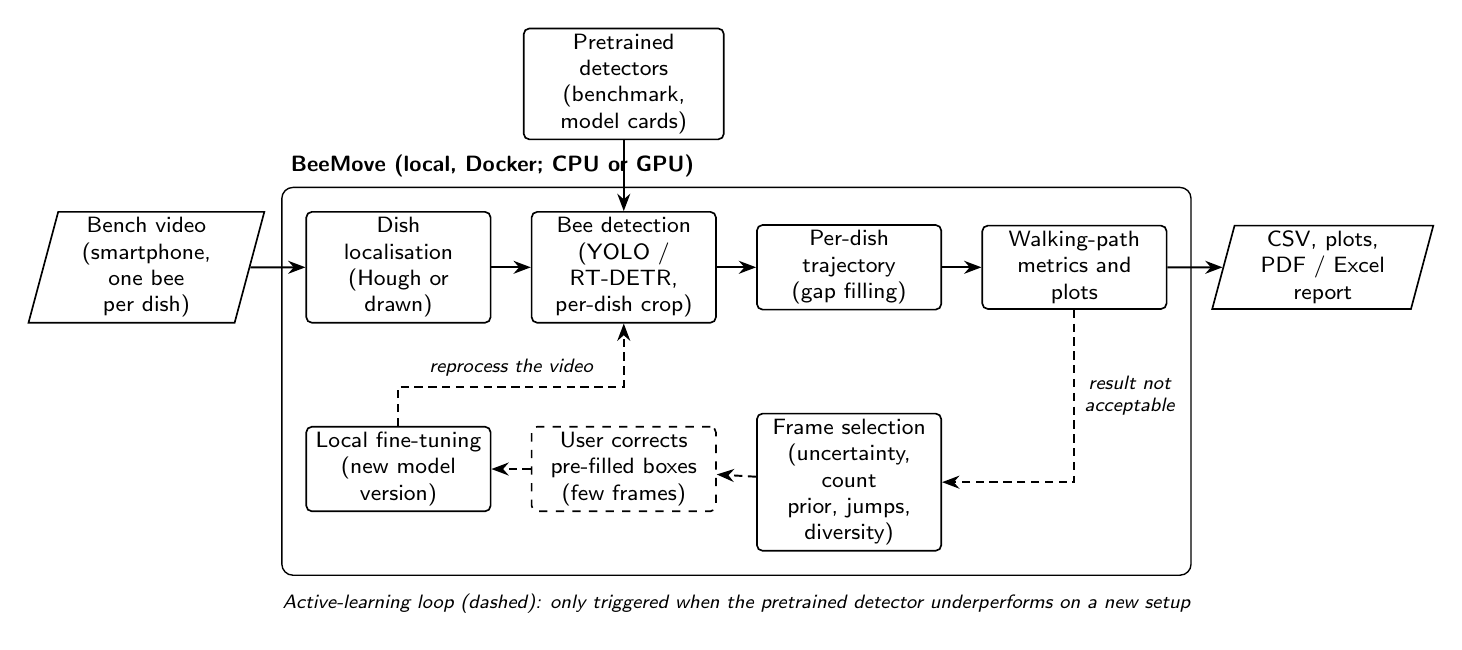
\begin{tikzpicture}[
  font=\footnotesize,
  >={Stealth[length=2.2mm]},
  box/.style={draw, rounded corners=2pt, align=center, minimum height=10mm,
              text width=22mm, inner sep=2pt, line width=0.6pt, fill=white},
  user/.style={box, dashed},
  io/.style={draw, align=center, text width=21mm, minimum height=10mm,
             inner sep=2pt, line width=0.6pt, trapezium, trapezium left angle=75,
             trapezium right angle=105, trapezium stretches body},
  flow/.style={->, line width=0.7pt},
  loop/.style={->, line width=0.7pt, densely dashed},
  lbl/.style={font=\scriptsize\itshape, align=center},
]

% ---------------------------------------------------------------- bench
\node[io] (video) {Bench video\\(smartphone,\\one bee per dish)};

% ---------------------------------------------------------------- pipeline
\node[box, right=7mm of video] (dishes) {Dish\\localisation\\(Hough or drawn)};
\node[box, right=5mm of dishes] (detect) {Bee detection\\(YOLO / RT-DETR,\\per-dish crop)};
\node[box, right=5mm of detect] (track) {Per-dish\\trajectory\\(gap filling)};
\node[box, right=5mm of track] (metrics) {Walking-path\\metrics and\\plots};
\node[io, right=7mm of metrics] (report) {CSV, plots,\\PDF / Excel\\report};

\draw[flow] (video) -- (dishes);
\draw[flow] (dishes) -- (detect);
\draw[flow] (detect) -- (track);
\draw[flow] (track) -- (metrics);
\draw[flow] (metrics) -- (report);

% ---------------------------------------------------------------- loop
\node[box, below=13mm of track] (select) {Frame selection\\(uncertainty, count\\prior, jumps, diversity)};
\node[user, below=13mm of detect] (correct) {User corrects\\pre-filled boxes\\(few frames)};
\node[box, below=13mm of dishes] (finetune) {Local fine-tuning\\(new model\\version)};

\draw[loop] (metrics.south) |- node[lbl, pos=0.25, right] {result not\\acceptable} (select.east);
\draw[loop] (select) -- (correct);
\draw[loop] (correct) -- (finetune);
\draw[loop] (finetune.north) -- ++(0,5mm) -| node[lbl, pos=0.25, above] {reprocess the video} (detect.south);

% ---------------------------------------------------------------- frames
\begin{scope}[on background layer]
  \node[draw, line width=0.5pt, rounded corners=4pt, inner sep=3mm,
        fit=(dishes)(metrics)(select)(finetune),
        label={[font=\footnotesize\bfseries, anchor=south west]north west:BeeMove (local, Docker; CPU or GPU)}] (tool) {};
\end{scope}
\node[lbl, below=1mm of tool.south, anchor=north] {Active-learning loop (dashed): only triggered when the pretrained detector underperforms on a new setup};

% ---------------------------------------------------------------- models
\node[box, text width=24mm, above=9mm of detect] (zoo) {Pretrained detectors\\(benchmark,\\model cards)};
\draw[flow] (zoo) -- (detect);

\end{tikzpicture}
\end{document}
